\documentclass[border=10pt,tikz]{standalone}
\usepackage{tikz}
\usetikzlibrary{positioning,arrows.meta,shapes}
\begin{document}
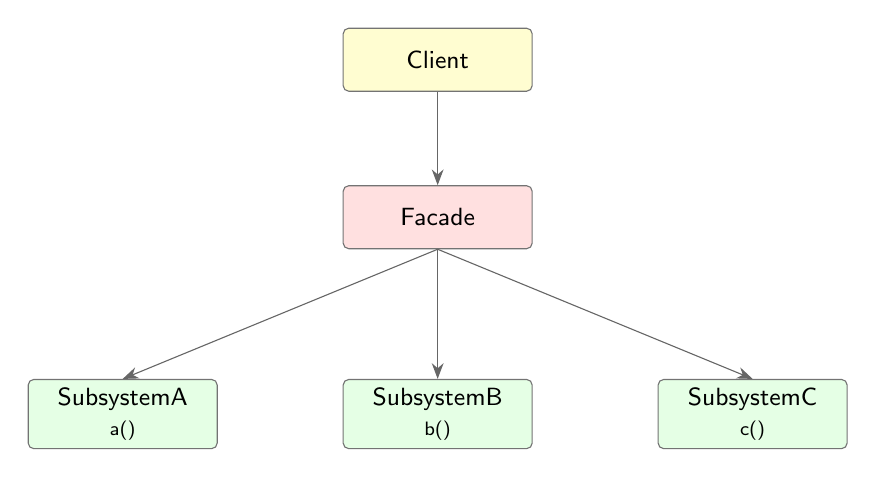
\begin{tikzpicture}[
  font=\sffamily\small,
  cls/.style={rectangle, rounded corners=2pt, draw=black!55, line width=0.4pt,
              minimum height=8mm, minimum width=24mm, inner sep=3pt, fill=white, align=center},
  con/.style={cls, fill=red!12},
  imp/.style={cls, fill=green!10},
  cli/.style={cls, fill=yellow!18},
  arr/.style={-{Stealth[length=2mm]}, draw=black!60}
]
\node[cli] (cl) at (0, 2.5) {Client};
\node[con] (f)  at (0, 0.5) {Facade};
\node[imp] (a)  at (-4,-2) {SubsystemA \\ \scriptsize a()};
\node[imp] (b)  at ( 0,-2) {SubsystemB \\ \scriptsize b()};
\node[imp] (c)  at ( 4,-2) {SubsystemC \\ \scriptsize c()};

\draw[arr] (cl) -- (f);
\draw[arr] (f.south) -- (a.north);
\draw[arr] (f.south) -- (b.north);
\draw[arr] (f.south) -- (c.north);
\end{tikzpicture}
\end{document}
